\section{Inference Queries}
We have seen two major types of compact representations of joint probability distributions in terms of graphs. Summarizing the expressions of the joint distribution, we can write
\begin{align}
\text{For UGM: }\Prob(x_1, \cdots, x_n) &= \dfrac{1}{Z}\prod_C \psi_C(x_C) \\
\text{For DGM: }\Prob(x_1, \cdots, x_n) &= \prod_i \Prob(x_i|\text{Pa}(x_i))
\end{align}
We get a very compact representation if $\text{Pa}(x_i)$ is small. \\
Given a probability distribution $P$, we can ask two major types of queries - 
\begin{enumerate}
	\item \textit{Marginal probability queries over a sm`all subset of variables: }Given $P$, what is the marginal probability of $x_1$?.
	\begin{equation}
	\begin{split}
		\Prob(x_1) &= \sum_{x_2, \cdots, x_n} \Prob(x_1, \cdots, x_n) \\
		&= \sum_{x_2=1}^m \cdots \sum_{x_n=1}^m \Prob(x_1, \cdots, x_n)
	\end{split}
	\end{equation}
We can see that if each variable takes $m$ values, then the brute-force computation of the marginal probability will take $\mathcal{O}(m^{n-1})$ time.
\item \textit{Most likely labels of remaining variables (MAP queries): }Here, we ask questions of the form,
\begin{equation}
	\mathbf{x}^* = \argmax_{x_1, \cdots, x_n} \Prob(x_1, \cdots, x_n)
\end{equation}
An example of such a query could be - find the most likely entity labels of all words in a sentence.
\end{enumerate}
\begin{exmp}[Exact Inference]
Say we have a probability distribution over three binary variables as 
\[P(x_1, x_2, x_3) = \dfrac{1}{Z}\psi_{12}(x_1, x_2)\psi_{23}(x_2, x_3)\]
\begin{marginfigure}
	\centering
	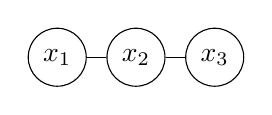
\begin{tikzpicture}[main/.style = {draw, circle}] 
		\node[main] (1) {$x_1$}; 
		\node[main] (2) [right of=1] {$x_2$}; 
		\node[main] (3) [right of=2] {$x_3$}; 
		\draw[-] (1) -- (2);
		\draw[-] (2) -- (3);
	\end{tikzpicture}
	\caption{UGM for $P(x_1, x_2, x_3)$}
	\label{fig:iq-p123-ugm}		
\end{marginfigure}
The UGM for this is shown in Figure \ref{fig:iq-p123-ugm}. Say we have the potential tables (each entry being $\psi_{ij}(a,b)$ representing the potential) as
\begin{center}
	\begin{tabular}{cc|c|c|}
		& \multicolumn{1}{c}{} & \multicolumn{2}{c}{$x_2$}\\
		& \multicolumn{1}{c}{} & \multicolumn{1}{c}{$0$}  & \multicolumn{1}{c}{$1$} \\\cline{3-4}
		\multirow{2}*{$x_1$}  & $0$ & $5$ & $2	$ \\\cline{3-4}
		& $1$ & $1$ & $4$ \\\cline{3-4}
	\end{tabular}
\qquad
\begin{tabular}{cc|c|c|}
	& \multicolumn{1}{c}{} & \multicolumn{2}{c}{$x_3$}\\
	& \multicolumn{1}{c}{} & \multicolumn{1}{c}{$0$}  & \multicolumn{1}{c}{$1$} \\\cline{3-4}
	\multirow{2}*{$x_2$}  & $0$ & $2$ & $10$ \\\cline{3-4}
	& $1$ & $5$ & $3$ \\\cline{3-4}
\end{tabular}
\end{center}
For example, we see that $\psi_{12}(0,0) = 5$. Let us find $P(x_1)$. 
\[P(x_1) =\dfrac{1}{Z} \sum_{x_2 \in \{0,1\}}\sum_{x_3 \in \{0,1\}}\psi_{12}(x_1, x_2)\psi_{23}(x_2, x_3)\]
We multiply the above two tables to get an intermediate potential distribution $\psi_{123}(x_1, x_2, x_3)$ and get a three dimensional table as follows (note that the columns denote $x_2$ and the rows denote $x_1$)
\begin{center}
	\begin{tabular}{cc|c|c|}
		& \multicolumn{1}{c}{} & \multicolumn{2}{c}{$x_3=0$}\\
		& \multicolumn{1}{c}{} & \multicolumn{1}{c}{$0$}  & \multicolumn{1}{c}{$1$} \\\cline{3-4}
		\multirow{2}*{}  & $0$ & $10$ & $10	$ \\\cline{3-4}
		& $1$ & $2$ & $20$ \\\cline{3-4}
	\end{tabular}
	\qquad
	\begin{tabular}{cc|c|c|}
		& \multicolumn{1}{c}{} & \multicolumn{2}{c}{$x_3=1$}\\
		& \multicolumn{1}{c}{} & \multicolumn{1}{c}{$0$}  & \multicolumn{1}{c}{$1$} \\\cline{3-4}
		\multirow{2}*{}  & $0$ & $50$ & $6$ \\\cline{3-4}
		& $1$ & $10$ & $12$ \\\cline{3-4}
	\end{tabular}
\end{center}
For example, $\psi_{12}(0,0)\psi_{23}(0,0) = 2\times5=10$. The next computation is to sum over $x_3$.
\[P(x_1) = \dfrac{1}{Z} \sum_{x_2 \in \{0,1\}} \psi_{12}^*(x_1, x_2)\]
The table after sum denoting $\psi_{12}^*(x_1, x_2)$ is
\begin{center}
	\begin{tabular}{cc|c|c|}
		& \multicolumn{1}{c}{} & \multicolumn{2}{c}{$x_2$}\\
		& \multicolumn{1}{c}{} & \multicolumn{1}{c}{$0$}  & \multicolumn{1}{c}{$1$} \\\cline{3-4}
		\multirow{2}*{$x_1$}  & $0$ & $60$ & $16$ \\\cline{3-4}
		& $1$ & $12$ & $32$ \\\cline{3-4}
	\end{tabular}
\end{center}
Now we eliminate $x_2$ by summing over the row values, thus finally
\[
\psi_1^*(x_1) = \dfrac{1}{Z}\begin{bmatrix}
	76 \\ 44
\end{bmatrix}
\]
Since this $P(x_1) = \psi_1^*(x_1)$, we immediately get to know that $Z = 76+44 = 120$. \\
Clearly, we see through the example that the calculation, even for three variables is cumbersome. Image doing this for thousands! \\
From the table in the above example, we can also calculate the assignment which gives the maximum probability. Note the $\psi_{123}$ table made, and see that $x_1=0, x_2=0, x_3=1$ has the score of $50$ giving the highest probability. But let us write this in a more algorithmic way
\[\mathbf{x^*} = \argmax_{x_2} \argmax_{x_2}\argmax_{x_3} \psi_{12}(x_1,x_2)\psi_{23}(x_2,x_3) \]
Let us construct the table $\psi_{12}^{\max} (x_1, x_2)$ from the $\psi_{123}$ table
\begin{center}
	\begin{tabular}{cc|c|c|}
		& \multicolumn{1}{c}{} & \multicolumn{2}{c}{$x_2$}\\
		& \multicolumn{1}{c}{} & \multicolumn{1}{c}{$0$}  & \multicolumn{1}{c}{$1$} \\\cline{3-4}
		\multirow{2}*{$x_1$}  & $0$ & $50$ for $x_3=1$ & $10$ for $x_3=0$ \\\cline{3-4}
		& $1$ & $10$ for $x_3=0$ & $20$ for $x_3=0$ \\\cline{3-4}
	\end{tabular}
\end{center}
Similarly, $\psi_1^{\max} (x_1)$ will be
\[
\begin{bmatrix}
	50 \text{ for $x_2=0, x_3=1$} \\ 20 \text{ for $x_2=1, x_3=0$} 
\end{bmatrix}
\]
At last, we can do an argmax over $x_1$ to get the assignment $x_1=0, x_2=0,x_3=1$ for the score of $50$.
\end{exmp}
Clearly, after the example, it is clear that we want to avoid the exponential overhead that brute-force approach applies.
\subsection{Exact Inference on Chains}
Consider the chain show in Figure \ref{fig:iq-chain}.
\begin{marginfigure}
	\centering
	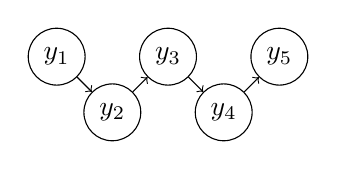
\begin{tikzpicture}[main/.style = {draw, circle}] 
		\node[main] (1) {$y_1$}; 
		\node[main] (2) [below right of=1] {$y_2$}; 
		\node[main] (3) [above right of=2] {$y_3$}; 
		\node[main] (4) [below right of=3] {$y_4$}; 
		\node[main] (5) [above right of=4] {$y_5$}; 
		\draw[->] (1) -- (2);
		\draw[->] (2) -- (3);
		\draw[->] (3) -- (4);
		\draw[->] (4) -- (5);
	\end{tikzpicture}
	\caption{Chain graph}
	\label{fig:iq-chain}		
\end{marginfigure}
We see that in the graph we would have potentials of the form $\psi_i(y_i, y_{i+1})$, and 
\begin{equation}
	\Prob(y_1, \cdots, y_n) = \prod_i \psi_i(y_i, y_{i+1})
\end{equation}
\textit{Note:} Since we don't have immoralities, the MRF is equivalent to the undirected version of the graph. Say we want to calculate 
\begin{equation}
\Prob(y_5=1) = \sum_{y_1, \cdots, y_4} \Prob(y_1, y_2, y_3, y_4, 1)
\end{equation}
The key idea to reducing computations is to push summations past the multiplications, i.e
\begin{equation}
\begin{split}
\Prob(y_5=1) &= \sum_{y_1, \cdots, y_4} \Prob(y_1, y_2, y_3, y_4, 1) \\
&= \sum_{y_1}\sum_{y_2}\sum_{y_3}\sum_{y_4} \psi_1(y_1, y_2)\psi_2(y_2,y_3)\psi_3(y_3,y_4)\psi_4(y_4,1) \\
&= \sum_{y_1}\sum_{y_2}\psi_1(y_1, y_2)\sum_{y_3}\psi_2(y_2, y_3)\sum_{y_4}\psi_3(y_3, y_4)\psi_4(y_4, 1) \\
&= \sum_{y_1}\sum_{y_2}\psi_1(y_1, y_2)\sum_{y_3}\psi_2(y_2, y_3)\mathcal{B}_3(y_3) \\
&= \sum_{y_1}\sum_{y_2}\psi_1(y_1, y_2) \mathcal{B}_2(y_2) \\
&= \sum_{y_1} \mathcal{B}_1(y_1) 
\end{split}
\end{equation}
We denote $\mathcal{B}_i(y_i)$ as the \textit{belief} which flows from node $i+1$ to $i$. This is an efficient computation. In general, if we have a chain with $n$ variables and each can take $m$ values, the above algorithm (breaking into beliefs) takes time in order of $\mathcal{O}(nm^2)$. \\
Notice that we did the efficient computation for chains, the natural question is, for what other graphs can this be done? \\
\begin{marginfigure}
	\centering
	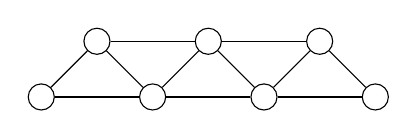
\begin{tikzpicture}[main/.style = {draw, circle}] 
		\node[main] (0) {};
		\node[main] (1) [above right of=0]{}; 
		\node[main] (2) [below right of=1] {}; 
		\node[main] (3) [above right of=2] {}; 
		\node[main] (4) [below right of=3] {}; 
		\node[main] (5) [above right of=4] {}; 
		\node[main] (6) [below right of=5] {}; 
		\draw[-] (0) -- (1);
		\draw[-] (1) -- (2);
		\draw[-] (0) -- (2);
		\draw[-] (1) -- (3);
		\draw[-] (2) -- (3);
		\draw[-] (2) -- (4);
		\draw[-] (3) -- (4);
		\draw[-] (3) -- (5);
		\draw[-] (4) -- (5);
		\draw[-] (4) -- (6);	
		\draw[-] (5) -- (6);
	\end{tikzpicture}
	\caption{Triangular graph}
	\label{fig:iq-triangle}		
\end{marginfigure}
Another one is shown in Figure \ref{fig:iq-triangle}. We define potential over each triangle (say $\psi_{123}$). If we follow a similar idea as the algorithm above, the time required for this computation will be $\mathcal{O}(nm^3)$.

\subsection{Hardness of Inference and 3-SAT}
The above discussion might lead to the thought that any graph $G$ which can be factorized into small clique sizes might have an efficient computation method (i.e polynomial time) of calculating the marginal probability.
\begin{marginfigure}
	\centering
	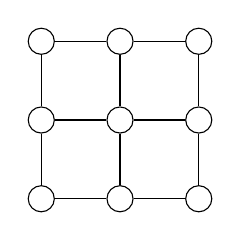
\begin{tikzpicture}[main/.style = {draw, circle}] 
		\node[main] (0) {};
		\node[main] (1) [right of=0]{}; 
		\node[main] (2) [right of=1] {}; 
		\node[main] (3) [below of=0] {}; 
		\node[main] (4) [below of=1] {}; 
		\node[main] (5) [below of=2] {}; 
		\node[main] (6) [below of=3] {}; 
		\node[main] (7) [below of=4] {}; 
		\node[main] (8) [below of=5] {}; 
		\draw[-] (0) -- (1);
		\draw[-] (1) -- (2);
		\draw[-] (0) -- (3);
		\draw[-] (1) -- (4);
		\draw[-] (2) -- (5);
		\draw[-] (3) -- (4);
		\draw[-] (5) -- (4);
		\draw[-] (3) -- (6);
		\draw[-] (4) -- (7);
		\draw[-] (5) -- (8);	
		\draw[-] (6) -- (7);
		\draw[-] (7) -- (8);
	\end{tikzpicture}
	\caption{Grid graph}
	\label{fig:iq-grid}		
\end{marginfigure}
 The answer sadly is no, and a counter example is the grid graph shown in Figure \ref{fig:iq-grid}. \\
 We will now reduce the $3$-SAT to inference in Bayesian Networks.
 \begin{defn}[$3$-SAT Problem]
 Given $n$ boolean variables $x_1, \cdots x_n$ such that $x_i \in \{T,F\}$. We define a literal $\ell$ to be the variable $x_i$ or its negation $\neg x_i$ or $\bar{x}_i$. Given a set of $K$ clauses $C_1, C_2, \cdots, C_K$ with each clause being
 \begin{equation} \label{eq:3-sat-clause}
 	C_j = \ell_{j_1} \lor \ell_{j_2} \lor \ell_{j_3}
 \end{equation}
The $3$-SAT problem is to decide if there exists an assignment of values to the $n$ variables such that 
\begin{equation}\label{eq:3-sat-sat}
	C_1 \land C_2 \land \cdots \land C_K = T
\end{equation}
 \end{defn}
\begin{exmp}\label{exmp:3-sat}
Consider $n=4, K=3$ and
\begin{align*}
	C_1 &= x_1 \lor \bar{x}_2 \lor \bar{x}_3 \\ 
	C_2 &= x_2 \lor x_3 \lor \bar{x}_4 \\
	C_3 &= x_4 \lor \bar{x}_1 \lor \bar{x}_2
\end{align*}
In this case, having all $x_i = T$ for $i = \{1, 2, 3, 4\}$ solves the problem.
\end{exmp}
In the above example, we by chance got lucky and solved the problem, but in general for a large number of variables, it is not possible to go over all possible combinations of values, since it requires an exponential amount of time. \\
Now we represent $3$-SAT as a Bayesian Network.
	\begin{marginfigure}
	\centering
	\begin{tikzpicture}[main/.style = {draw, circle}] 
		\node[main] (x1) {$x_1$}; 
		\node[main] (x2) [right of=x1] {$x_2$};
		\node[main] (x3) [right of=x2] {$x_3$};
		\node[main] (x4) [right of=x3] {$x_4$};
		\node[main] (c1) [below = of $(x1)!0.5!(x2)$] {$C_1$};
		\node[main] (c2) [below = of $(x2)!0.5!(x3)$] {$C_2$};
		\node[main] (c3) [below = of $(x3)!0.5!(x4)$] {$C_3$};
		\node[main] (s) [below = of c2] {$\mathcal S$};
     	\draw[->] (x1) -- (c1);
     	\draw[->] (x2) -- (c1);
     	\draw[->] (x3) -- (c1);
     	\draw[->] (x2) -- (c2);
     	\draw[->] (x3) -- (c2);
     	\draw[->] (x4) -- (c2);
     	\draw[->] (x4) -- (c3);
     	\draw[->] (x1) -- (c3);
     	\draw[->] (x2) -- (c3);
     	\draw[->] (c1) -- (s);
     	\draw[->] (c2) -- (s);
     	\draw[->] (c3) -- (s);
	\end{tikzpicture}
	\caption{3-SAT as BN}
	\label{fig:bn-3-sat}
\end{marginfigure}
Let us do that in a \textit{layer} sense. Let the first layer have all the variables as nodes and the next layer have all the clauses. Each clause will have 3 parents due to Equation \ref{eq:3-sat-clause}. Finally, the third layer would have $\mathcal S$, which is the satisfiability (Equation \ref{eq:3-sat-sat}), and it's parents would be all the clauses. Figure \ref{fig:bn-3-sat} shows the BN of Example \ref{exmp:3-sat}. \\
Coming back to the general setting, for each variable $x_i$, we denote
\begin{equation}
	\Prob(x_i) = \begin{cases}
		\frac{1}{2} & x_i=F \\
		\frac{1}{2} & x_i=T
	\end{cases}
\end{equation}

We also need to define $\Prob(C_j|\ell_{j_1}, \ell_{j_2}, \ell_{j_3})$. To do this, we assign a non-zero probability to only those which make $C_j=T$. This can be done uniformly (say out of the 8 assignments, 5 give a non-zero value, then $1$ for each of those assignments, and $0$ to rest - this is done because each $C_j$ is a deterministic function of the literals). Finally, we write the last probability $\Prob(\mathcal S|C_1, \cdots, C_K)$ as $1$ if $C_1, \cdots, C_K = T$, i.e all are true, and in the rest of the cases, we assign it as zero (note the difference here - the table for each $C_i$ had 8 rows, and the table for $\mathcal S$ has $2^K$ rows). The $2^K$ shows that it is not polynomial. This is again, not efficient. \\
One small change we can do is that instead of having a single $\mathcal S$ in the last layer, have $K-1$, such that each $\mathcal{S}_i$ is connected to $C_{i-1}$ and $C_i$ as parents, and each $\mathcal{S}_i$ is a parent of $\mathcal{S}_{i+1}$. This allows us to create the probability table as $\Prob(\mathcal{S}_j | \mathcal{S}_{j-1}, C_{j-1}, C_j)$ which represents the logic
\begin{equation}
	\mathcal{S}_j =  \mathcal{S}_{j-1} \land C_{j-1} \land C_j 
\end{equation} 
This allows each $\mathcal{S}_j$ with 8 variables, bringing in the needed efficiency. More specifically, the space required now is polynomial, since each $S_j$ requires only $2^4$ space, each $C_j$ requires $2^5$ space and each $x_j$ requires just constant (2) space. Thus overall the space required is $\mathcal{O}((K-1)\cdot2^4 + K\cdot 2^5+2)$
\\
Finally, if we can answer $\Prob(\mathcal{S}_j=1) > 0$ positively, then we know that a $3$-SAT assignment exists, else it does not.
\subsection{Variable Elimination on General Graphs}
We saw that using brute-force (i.e an exponential number of operations), we could calculate the normalizer $Z$. This is impractical, and hence we need a more efficient way to do so. Let's define the problem again - \\
Given an arbitrary set of potentials $\psi_C(x_C)$ in a graph $G$ where $C$ are the cliques in $G$, we need to find 
\[ Z = \sum_{x_1,\cdots,x_n} \prod_C \psi_C(x_C)\]
The algorithm to do so is as follows: \\
\begin{algorithm}[H]\label{alg:var-elim}
	\DontPrintSemicolon
	\textbf{Input:} Graph $G$\;
	\textbf{Variables:} $x_1, x_2, \cdots, x_n$ present in a \textit{good} ordering\;
	$\mathcal F \longleftarrow \{\psi_C(x_C)$ where $C=$ cliques in $G$\}  \;
	\For{$i=1$ to $n$}{
		$\mathcal F_i \longleftarrow$ factors in $\mathcal F$ containing $x_i$\;
		$\mathcal M_i \longleftarrow$ product of factors in $\mathcal F_i$\;
		$m_i \longleftarrow \sum_{x_i} \mathcal M_i$\;
		$\mathcal{F \longleftarrow (F}-\mathcal{F}_i) \cup \{m_i\}$\;
	}
	\caption{Variable Elimination}
\end{algorithm}
At the end, $\mathcal F$ consists of only a constant. Note that the product of factors isn't trivial, i.e we would need to multiply probability tables. To understand Algorithm \ref{alg:var-elim}, let's see an example.
\begin{exmp}\label{exmp:var-elim}
Say we have been given 5 variables, and the cliques are
\[\psi_{12}(x_1, x_2), \psi_{24}(x_2, x_4), \psi_{23}(x_2, x_3), \psi_{45}(x_4, x_5), \psi_{35}(x_3, x_5)\]
\begin{marginfigure}
	\centering
	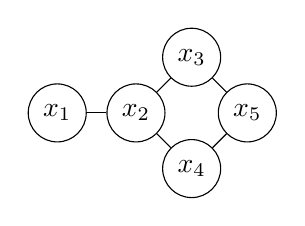
\begin{tikzpicture}[main/.style = {draw, circle}] 
		\node[main] (4) {$x_4$}; 
		\node[main] (2) [above left of=4] {$x_2$}; 
		\node[main] (5) [above right of=4] {$x_5$}; 
		\node[main] (3) [above right of=2] {$x_3$}; 
		\node[main] (1) [left of=2] {$x_1$}; 
		\draw[-] (1) -- (2);
		\draw[-] (2) -- (3);
		\draw[-] (2) -- (4);
		\draw[-] (4) -- (5);
		\draw[-] (3) -- (5);
	\end{tikzpicture}
	\caption{UGM for Example}
	\label{fig:iq-var-elim}		
\end{marginfigure}
The corresponding graph is in Figure \ref{fig:iq-var-elim}. We can see that 
\[Z = \sum_{x_1 \cdots x_5}\psi_{12}(x_1 x_2) \psi_{24}(x_2 x_4) \psi_{23}(x_2 x_3) \psi_{45}(x_4 x_5) \psi_{35}(x_3 x_5)\]
Say our good ordering is $x_1, x_2, x_3, x_4, x_5$. So we start
\begin{itemize}
	\item[$\diamond$] First variable $x_1$ - 
	\begin{align*}
	\mathcal{F}_1 &= \{\psi_{12}(x_1, x_2)\} \\
	\mathcal{M}_1(x_1, x_2) &= \psi_{12}(x_1, x_2) \\
	m_1(x_2) &= \sum_{x_1}\mathcal{M}_1 \\
	\mathcal{F} &= \{\psi_{24}(x_2, x_4), \psi_{23}(x_2, x_3), \psi_{45}(x_4, x_5), \psi_{35}(x_3, x_5), m_1(x_2)\}
	\end{align*}
\item[$\diamond$] Second variable $x_2$ - 
\begin{align*}
	\mathcal{F}_2 &= \{\psi_{24}(x_2, x_4), \psi_{23}(x_2, x_3), m_1(x_2)\} \\
	\mathcal{M}_2(x_2, x_3, x_4) &= \psi_{12}(x_2, x_4)\psi_{23}(x_2, x_3) m_1(x_2) \\
	m_2(x_3, x_4) &= \sum_{x_2}\mathcal{M}_2 \\
	\mathcal{F} &= \{\psi_{45}(x_4, x_5), \psi_{35}(x_3, x_5), m_2(x_3, x_4)\}
\end{align*}
\item[$\diamond$] Third variable $x_3$ - 
\begin{align*}
	\mathcal{F}_3 &= \{\psi_{35}(x_3, x_5), m_2(x_3, x_4)\} \\
	\mathcal{M}_3(x_3, x_4, x_5) &= \psi_{35}(x_3, x_5) m_2(x_3, x_4) \\
	m_3(x_4, x_5) &= \sum_{x_3}\mathcal{M}_3 \\
	\mathcal{F} &= \{\psi_{45}(x_4, x_5), m_3(x_4, x_5)\}
\end{align*}
\item[$\diamond$] Fourth variable $x_4$ - 
\begin{align*}
	\mathcal{F}_4 &= \{\psi_{45}(x_4, x_5), m_3(x_4, x_5)\} \\
	\mathcal{M}_4(x_4, x_5) &= \psi_{45}(x_4, x_5)m_3(x_4, x_5) \\
	m_4(x_5) &= \sum_{x_4}\mathcal{M}_4 \\
	\mathcal{F} &= \{m_4(x_5)\}
\end{align*}
\end{itemize}
\end{exmp}
The above example showed how $\mathcal F$ is a singleton set at the end. We can also modify Algorithm \ref{alg:var-elim} to get $\Prob(x_i)$ as follows - 
\begin{itemize}
	\item[$\diamond$] In line $1$ of Algorithm \ref{alg:var-elim}, we choose a good ordering such that $x_i$ is last
	\item[$\diamond$] The for loop in line 3 runs only for $n-1$ iterations
	\item[$\diamond$] After this, at the end, $\mathcal F$ will consist of unnormalized values, sum of which will give $Z$, and each term divided by $Z$ will give the required probability.
\end{itemize}
What if we want to compute the MAP query? For that, we do the follwing - 
\begin{itemize}
	\item[$\diamond$] In line 6, we have $\hat{m}_i = \max_{x_i} \mathcal{M}_i$ and we have to keep around the maximizing assignment
	\item[$\diamond$] In the end $\mathcal F$ consists of the required argmax.
\end{itemize}
\begin{thm}
The complexity of the Variable Elimination algorithm is $\mathcal{O}(nm^w)$ where $w$ is the maximum number of variables in any factor.
\end{thm}
\begin{proof}[Sketch of proof]
The bottleneck step in the algorithm's for loop is computing the product of factors, and in general if the factor has $\kappa$ variables, then the time to do the product will be $\mathcal{O}(m^\kappa)$.
\end{proof}
In Example \ref{exmp:var-elim}, we see that the time complexity is $\mathcal{O}(nm^3)$. If we started with $x_2$, our time complexity would've been $\mathcal{O}(nm^4)$.
\begin{marginfigure}
	\centering
	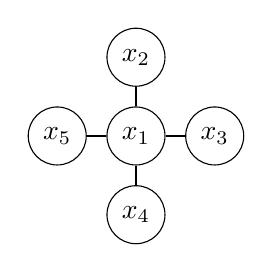
\begin{tikzpicture}[main/.style = {draw, circle}] 
		\node[main] (1)  {$x_1$}; 
		\node[main] (4) [below of=1]{$x_4$}; 
		\node[main] (2) [above of=1] {$x_2$}; 
		\node[main] (3) [ right of=1] {$x_3$}; 
		\node[main] (5) [ left of=1] {$x_5$}; 
		\draw[-] (1) -- (2);
		\draw[-] (1) -- (3);
		\draw[-] (1) -- (4);
		\draw[-] (1) -- (5);
		\draw[-] (1) -- (5);
	\end{tikzpicture}
	\caption{Star Graph}
	\label{fig:iq-star-graph}		
\end{marginfigure}
More interestingly, if we have a star graph (Figure \ref{fig:iq-star-graph}), and if we start with the centre node first, we encounter a very severe penalty in terms of time complexity. This elimination order will give you $\mathcal O(m^n)$ running time, while removing the non-central nodes first gives you just $\mathcal{O}(nm^2)$ running time.\\
Unfortunately, choosing the optimal elimination order is NP hard in general. But for chordal (triangulated) graphs, the algorithm is polynomial time. But another problem we stumble upon is that if our graph is not triangular, optimal triangulation is NP hard (but there exist many heuristics to do this in polynomial time).
\begin{defn}[Simplicial]
A vertex in a graph $G$ is simplicial if its neighbors form a complete set.
\end{defn}
\begin{thm}
Every triangulated graph is either complete or has at least two non-adjacent simplicial vertices.
\end{thm}
\begin{proof}
To be added.
\end{proof}
The goal is to find an optimal ordering for inferring $\Prob(x_1)$, which means $x_1$ should be last.\\
\begin{algorithm}[H]\label{alg:opt-order}
	\DontPrintSemicolon
	\textbf{Input:} Graph $G$, $n=$ number of vertices in $G$\;
	\For{$i=1$ to $n$}{
		$\pi_i \longleftarrow$ any simplicial vertiex in $G$ except $1$\;
		Remove $\pi_i$ from $G$\;
	}
	\Return{ordering $\pi_1, \cdots, \pi_{n-1}$}
	\caption{Optimal ordering for triangulated graph}
\end{algorithm}
\begin{marginfigure}
	\centering
	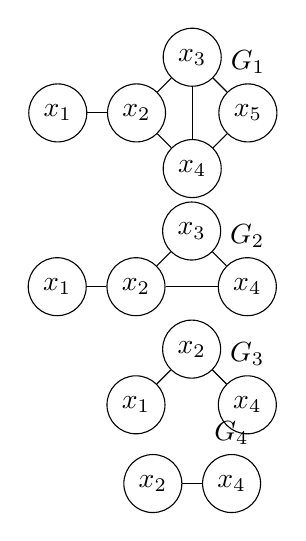
\begin{tikzpicture}[main/.style = {draw, circle}] 
		\begin{scope}
		\node[main] (4) {$x_4$}; 
		\node[main] (2) [above left of=4] {$x_2$}; 
		\node[main] (5) [above right of=4, label=$G_1$] {$x_5$}; 
		\node[main] (3) [above right of=2] {$x_3$}; 
		\node[main] (1) [left of=2] {$x_1$}; 
		\draw[-] (1) -- (2);
		\draw[-] (2) -- (3);
		\draw[-] (2) -- (4);
		\draw[-] (4) -- (5);
		\draw[-] (3) -- (5);
		\draw[-] (3) -- (4);
		\end{scope}
		\begin{scope}[yshift=-1.5cm, xshift=0.7cm]
		\node[main] (4) [label=$G_2$]{$x_4$}; 
		\node[main] (3) [above left of=4] {$x_3$}; 
		\node[main] (2) [below left of=3] {$x_2$}; 
		\node[main] (1) [left of=2] {$x_1$}; 
		\draw[-] (1) -- (2);
		\draw[-] (2) -- (3);
		\draw[-] (2) -- (4);
		\draw[-] (3) -- (4);
		\end{scope}
		\begin{scope}[yshift=-3cm, xshift=0.7cm]
			\node[main] (4) [label=$G_3$]{$x_4$}; 
			\node[main] (2) [above left of=4] {$x_2$}; 
			\node[main] (1) [below left of=2] {$x_1$}; 
			\draw[-] (1) -- (2);
			\draw[-] (2) -- (4);
		\end{scope}
	\begin{scope}[yshift=-4cm, xshift=-0.5cm]
		\node[main] (2){$x_2$}; 
		\node[main] (4) [label=$G_4$][right of=2] {$x_4$}; 
		\draw[-] (4) -- (2);
	\end{scope}
	\end{tikzpicture}
\caption{Sequence of graphs}
\label{fig:iq-opt-order}		
\end{marginfigure}
\begin{exmp}
Consider the triangulated graph $G_1$ given on the right for which we have to find the optimal ordering. We go over the iterations as follows
\begin{enumerate}
	\item  In $G_1$, we have $x_1$ and $x_5$ as simplicial vertices. Say we remove $x_5$ first, to get $G_2$.
	\item In $G_2$, we have $x_1, x_3$ and $x_4$ as the simplicial vertices. Say we remove $x_3$ to get $G_3$.
	\item In $G_3$, we have $x_1$ and $x_4$ as simplicial vertices. Say we remove $x_1$ to get $G_4$.
	\item In $G_4$ we have $x_2$ and $x_4$ as simplicial vertices.
	Say we remove $x_2$.
\end{enumerate}
The sequence of graphs is shown in Figure \ref{fig:iq-opt-order}. \\
Thus, finally we get the ordering $x_5, x_3, x_1, x_4, x_2$ as an optimal ordering. 
\end{exmp}
\subsection{Multiple Inference Queries}
The above subsection showed how we can calculate the optimal ordering and a single inference query. But say, we have been given a chain graph with potentials as $\psi_{i,i+1}(x_i, x_{i+1})$, say we need all $\Prob(x_1), \cdots, \Prob(x_n)$, can we do that faster? A no-brain method would be to use variable elimination $n$ times to get $\mathcal{O}(n^2m^2)$.
\begin{marginfigure}
	\centering
	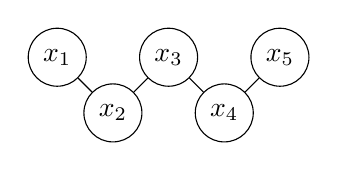
\begin{tikzpicture}[main/.style = {draw, circle}] 
		\node[main] (1) {$x_1$}; 
		\node[main] (2) [below right of=1] {$x_2$}; 
		\node[main] (3) [above right of=2] {$x_3$}; 
		\node[main] (4) [below right of=3] {$x_4$}; 
		\node[main] (5) [above right of=4] {$x_5$}; 
		\draw[-] (1) -- (2);
		\draw[-] (2) -- (3);
		\draw[-] (3) -- (4);
		\draw[-] (4) -- (5);
	\end{tikzpicture}
	\caption{Chain graph}
	\label{fig:iq-chain-graph}		
\end{marginfigure}
Say I have the chain graph in Figure \ref{fig:iq-chain-graph}. If we need to calculate $\Prob(x_1)$, we first remove $x_5$. This is followed by removing $x_4$, $x_3$ and $x_2$. \\
Now if we want to calculate $\Prob(x_2)$. We can reuse the computation done in removing $x_5, x_4$ and $x_3$. \\
We will see that if we skillfully reuse such computation, if each variable elimination run takes time $\mathfrak T$, the time for $n$ inference queries will take just $2\mathfrak T$.
\begin{rem}
Refer to Example \ref{exmp:var-elim}. In this notice that the arguments of $\mathcal M_i (\cdot)$ are cliques with \textit{induced} edges. For example, we have $\mathcal{M}_1(x_1, x_2)$ and clearly $\{x_1, x_2\}$ forms a clique. Second, we have $\mathcal{M}_2(x_2, x_3, x_4)$ and notice that when we add or \textit{induce} an edge between $x_2$ and $x_3$, $\{x_2, x_3, x_4\}$ forms a clique. This can be extended to all $\mathcal{M}_i(\cdot)$. For our notion of reusing, we are interested in the maximal cliques formed, and you can check that they refer to the cliques formed by the arguments of $\mathcal{M}_1, \mathcal{M}_2$ and $\mathcal{M}_3$.
\end{rem}
\subsection{Junction Trees}
The junction tree algorithm is an optimal general-purpose algorithm for \textbf{exact} marginal or MAP queries, and can simultaneously compute many such queries. It utilizes efficient data structures and overall has a complexity of $\mathcal O(m^wN)$ where $w$ is the size of the largest clique in the triangulated graph and each variable can take $m$ values. It is to note that 
\begin{itemize}
	\item[$\diamond$] Viterbi algorithm of Hidden Markov Models
	\item[$\diamond$] Forward-backward algorithm of Kalman Filters
\end{itemize}
are special cases of junction trees.
\begin{marginfigure}
	\centering
	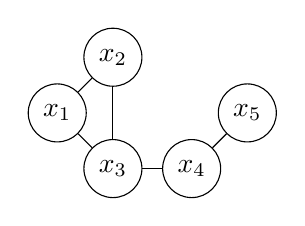
\begin{tikzpicture}[main/.style = {draw, circle}] 
		\node[main] (1)  {$x_1$}; 
		\node[main] (3) [below right of=1]{$x_3$}; 
		\node[main] (2) [above right of=1] {$x_2$}; 
		\node[main] (4) [right of=3] {$x_4$}; 
		\node[main] (5) [above right of=4] {$x_5$}; 
		\draw[-] (1) -- (2);
		\draw[-] (1) -- (3);
		\draw[-] (2) -- (3);
		\draw[-] (3) -- (4);
		\draw[-] (4) -- (5);
	\end{tikzpicture}
	\caption{Sample graph for JT}
	\label{fig:iq-jt-graph}		
\end{marginfigure}
\begin{defn}[Junction Tree]
Junction tree JT of a triangulated graph $G$ with nodes $x_1, \cdots, x_n$ is a tree where the nodes are the maximal cliques of $G$ and the edges obey the \textit{running intersection property}. This property states that if any two nodes contain variable $x_i$, then $x_i$ is present in every node in the unique path between them.
\end{defn}
\begin{marginfigure}
	\centering
	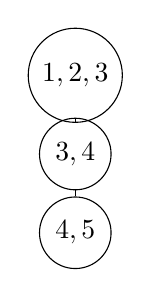
\begin{tikzpicture}[main/.style = {draw, circle}] 
		\node[main] (123)  {$1,2,3$}; 
		\node[main] (34) [below of=123]{$3,4$}; 
		\node[main] (45) [below of=34] {$4,5$}; 
		\draw[-] (123) -- (34);
		\draw[-] (34) -- (45);
	\end{tikzpicture}
	\caption{Junction Tree example}
	\label{fig:iq-jt-graph-jt}		
\end{marginfigure}
\begin{exmp}
For the graph given in Figure \ref{fig:iq-jt-graph}, we have the maximal cliques as $\{x_1, x_2, x_3\}, \{x_3, x_4\}, \{x_4, x_5\}$. Thus, the junction tree for the graph is given in Figure \ref{fig:iq-jt-graph-jt}
\end{exmp}
\begin{thm}
A graph will have a junction tree if and only if it is chordal.
\end{thm}
\begin{proof}
Skipped.
\end{proof}
\noindent\textbf{Construction of a junction tree}\\
If our graph is chordal, we have efficient polynomial time algorithms to create a JT. We first enumerate a set of maximal cliques covering our graph $G$, then we connect the cliques to get a tree satisfying the \textit{running intersection property}. Note that if our graph is non-triangulated, we need to triangulate it first using heuristics, since optimal triangulation is NP-hard.
\begin{defn}[Optimal triangulation]
A triangulation which gives rise to a JT where the size of the largest clique is smallest is called the optimal triangulation.
\end{defn}
\noindent A general method for finding heuristics is -
\begin{verbatim}
for i = 1 to n
	choose the vertex for which some score is minimum
	connect all neighbors of chosen vertex
	remove the chosen vertex from the graph
\end{verbatim}
Some heuristics of triangulation are
\begin{enumerate}
	\item Choose the vertex with smallest degree and connect all its neighbors
	\item Chose the vertex which will require the smallest number of edges to connect neighbors
\end{enumerate}
\begin{exmp}\label{exmp:jt-creation}
	Creation of a JT from a UGM:
	\begin{enumerate}
		\begin{marginfigure}
			\centering
			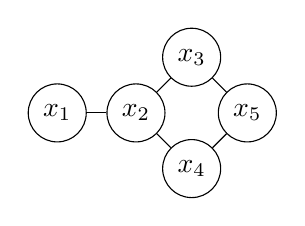
\begin{tikzpicture}[main/.style = {draw, circle}] 
				\node[main] (1)  {$x_1$}; 
				\node[main] (2) [right of=1] {$x_2$};
				\node[main] (3) [above right of=2]{$x_3$};  
				\node[main] (4) [below right of=2] {$x_4$}; 
				\node[main] (5) [above right of=4] {$x_5$}; 
				\draw[-] (1) -- (2);
				\draw[-] (2) -- (3);
				\draw[-] (2) -- (4);
				\draw[-] (3) -- (5);
				\draw[-] (4) -- (5);
			\end{tikzpicture}
			\caption{Non-chordal graph}
			\label{fig:iq-jt-exmp-unchordal}	
		\end{marginfigure}
	\begin{marginfigure}
		\centering
		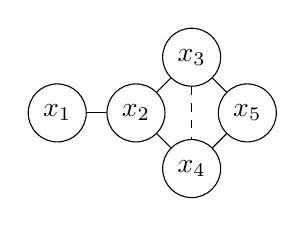
\begin{tikzpicture}[main/.style = {draw, circle}] 
			\node[main] (1)  {$x_1$}; 
			\node[main] (2) [right of=1] {$x_2$};
			\node[main] (3) [above right of=2]{$x_3$};  
			\node[main] (4) [below right of=2] {$x_4$}; 
			\node[main] (5) [above right of=4] {$x_5$}; 
			\draw[-] (1) -- (2);
			\draw[-] (2) -- (3);
			\draw[-] (2) -- (4);
			\draw[-] (3) -- (5);
			\draw[-] (4) -- (5);
			\draw[dashed] (3) -- (4);
		\end{tikzpicture}
		\caption{Chordal graph}
		\label{fig:iq-jt-exmp-chordal}	
	\end{marginfigure}
\begin{marginfigure}
	\centering
	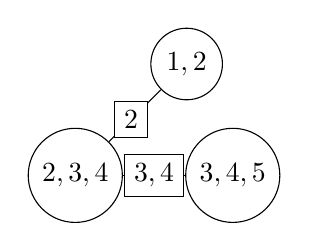
\begin{tikzpicture}[main/.style = {draw, circle}, sep/.style= {draw, rectangle}] 
		\node[main] (12)  {$1,2$}; 
		\node[sep] (2)  [below left of=12]{$2$}; 
		\node[main] (234) [below left of=2] {$2,3,4$};
		\node[sep] (34)  [right of=234]{$3,4$}; 
		\node[main] (345) [right of=34] {$3,4,5$};
		\draw[-] (12) -- (2);
		\draw[-] (2) -- (234);
		\draw[-] (234) -- (34);
		\draw[-] (34) -- (345);
	\end{tikzpicture}
	\caption{Clique-node graph}
	\label{fig:iq-jt-exmp-cliques}	
\end{marginfigure}
		\item Consider the graph in Figure \ref{fig:iq-jt-exmp-unchordal} as our starting graph. 
		
		\item We triangulate the graph to get the graph in Figure \ref{fig:iq-jt-exmp-chordal}. Notice that the maximal cliques are $C_1=\{x_1, x_2\}, C_2= \{x_2, x_3, x_4\}$ and $C_3=\{x_3, x_4, x_5\}$.
		
		\item These cliques act as nodes in our junction tree, and we connect the three cliques such that they satisfy the running intersection property. I have dropped the $x$ and just written the indices to avoid clutter. Note in Figure \ref{fig:iq-jt-exmp-cliques} that now we have two types of nodes - in circle we have the cliques, and in rectangles we have the \textit{separators}. Separators are variables present in the intersection of the nodes, thus
		\begin{equation}
		\text{Separator}(C_i, C_j) = C_i \cap C_j
		\end{equation}
	
		\item Now we assign potentials to all cliques. Note that from Example \ref{exmp:var-elim}, we had potentials $\psi_{12}, \psi_{23}, \psi_{24}, \psi_{35},\psi_{45}$. Thus here we can assign $\psi_{12}$ to $C_1$, $\psi_{23}, \psi_{24}$ to $C_2$ and $\psi_{35}, \psi_{45}$ to $C_3$. 
		\begin{rem}
		If we encounter any ambiguity in assigning potentials, i.e we can assign potentials to more than once clique-node, then we can arbitrarily assign it to any one.
		\end{rem}
	\end{enumerate}
\end{exmp}
\begin{thm}
Every triangulated graph has a simplicial vertex.
\end{thm}
\begin{proof}
Skipped.
\end{proof}
We now state the algorithm to find the maximal cliques in a triangulated graph \\
\begin{algorithm}[H]\label{alg:cliques-chordal}
	\DontPrintSemicolon
	\textbf{Input:} Triangulated graph $G$, $n=$ number of vertices in $G$\;
	\For{$i=1$ to $n$}{
		$\pi_i \longleftarrow$ any simplicial vertiex in $G$\;
		$C_i \longleftrightarrow \{\pi_i\} \cup \mathcal{N}(\pi_i)$\;
		Remove $\pi_i$ from $G$\;
	}
	\Return{the maximal cliques from $C_1, \cdots, C_n$}
	\caption{Finding maximal cliques in a chordal graph}
\end{algorithm}
\begin{thm}
A clique tree that satisfies the running intersection property maximized the number of separator variables.
\end{thm}
\begin{proof}
To be added.
\end{proof}
\begin{algorithm}[H]\label{alg:cliques-jt}
	\DontPrintSemicolon
	\textbf{Input:} Cliques $C_1, \cdots, C_k$\;
	Form a complete weighted graph $H$ with cliques as nodes and edge weights = size of the intersection of the two cliques it connects \;
	$T \longleftarrow$ maximum weight spanning tree of $H$\;
	\Return{$T$ as the junction tree}
	\caption{Forming a junction tree from a clique-node graph}
\end{algorithm}
Note that once we have the clique graph, we can make a weighted clique graph from that by adding $|\mathcal S|$ as the weight for each each between $C_i$ and $C_j$ where $\mathcal S = C_i \cap C_j$, and the problem of finding the junction tree boils down to finding the maximum weight spanning tree of the weighted graph.
\begin{exmp}
\begin{marginfigure}
	\centering
	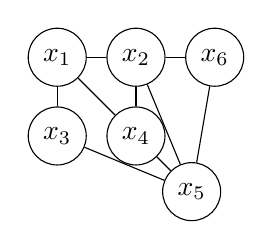
\begin{tikzpicture}[main/.style = {draw, circle}] 
		\node[main] (1)  {$x_1$}; 
		\node[main] (2) [right of=1] {$x_2$};
		\node[main] (3) [below of=1] {$x_3$};
		\node[main] (4) [below of=2] {$x_4$};
		\node[main] (5) [below right of=4] {$x_5$};
		\node[main] (6) [right of=2] {$x_6$};
		\draw[-] (1) -- (2);
		\draw[-] (1) -- (3);
		\draw[-] (1) -- (4);
		\draw[-] (2) -- (4);
		\draw[-] (2) -- (5);
		\draw[-] (2) -- (6);
		\draw[-] (3) -- (5);
		\draw[-] (4) -- (5);
		\draw[-] (5) -- (6);
	\end{tikzpicture}
	\caption{Undirected graph}
	\label{fig:iq-jt-exmp-ugm}	
\end{marginfigure}
Consider the undirected graph $H$ in Figure \ref{fig:iq-jt-exmp-ugm}. Say the potentials are defined over cliques of size 2. \\
To triangulate, say we pick a heuristic - smallest degree first. Start with $x_6$ and notice that its neighbors $x_2$ and $x_5$ are connected. Next we choose $x_3$ and connect $x_1$ and $x_5$. You can go on further, but notice that the graph is already triangulated (since on removing $x_1$ the graph becomes complete). Thus an ordering we can have is
\[x_6, x_3, x_1, x_2, x_5, x_4\]
Next we choose the maximal cliques. This can be done using Algorithm \ref{alg:cliques-chordal}. This gives the set of maximal cliques as
\begin{align*}
	C_1 &= \{x_3, x_1, x_5\}\\
	C_2 &= \{x_6, x_2, x_5\}\\
	C_3 &= \{x_1, x_2, x_4, x_5\}
\end{align*}
\begin{marginfigure}
	\centering
	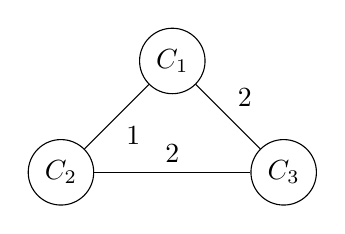
\begin{tikzpicture}[main/.style = {draw, circle}, node distance=2cm] 
		\node[main] (1)  {$C_1$}; 
		\node[main] (2) [below left of=1] {$C_2$};
		\node[main] (3) [below right of=1] {$C_3$};
		\draw[-] (1) to node[auto] {1} (2) ;
		\draw[-] (1) to node[auto] {2} (3) ;
		\draw[-] (2) to node[auto] {2} (3) ;
	\end{tikzpicture} 	
	\caption{Complete Weighted Graph}
	\label{fig:iq-jt-exmp-cwg}	
\end{marginfigure}
We then make the complete weighted graph as in Figure \ref{fig:iq-jt-exmp-cwg}. Clearly by removing the edge $C_1 - C_2$, we get the maximum spanning tree, and that gives the junction tree as shown in Figure \ref{fig:iq-jt-exmp-jt}.
\begin{marginfigure}
	\centering
	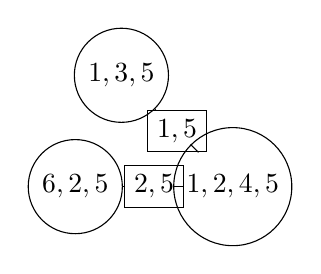
\begin{tikzpicture}[main/.style = {draw, circle}, sep/.style= {draw, rectangle}] 
		\node[main] (135)  {$1,3,5$}; 
		\node[sep] (5)  [below right of=135]{$1,5$}; 
		\node[main] (1245) [below right of=5] {$1, 2,4,5$};
		\node[sep] (25)  [left of=1245]{$2,5$}; 
		\node[main] (625) [left of=25] {$6, 2, 5$};
		\draw[-] (135) -- (5);
		\draw[-] (5) -- (1245);
		\draw[-] (625) -- (25);
		\draw[-] (25) -- (1245);
	\end{tikzpicture}
	\caption{Junction Tree}
	\label{fig:iq-jt-exmp-jt}	
\end{marginfigure}
To assign the potentials, we can assign $\psi_{13}, \psi_{35}$ to $C_1$, $\psi_{14}, \psi_{12}, \psi_{45}, \psi_{24}$ to $C_3$ and finally $\psi_{25}, \psi_{26}$ to $C_2$. The potential of a clique is the product of the potentials assigned to it.
\end{exmp}
\subsection{Message Passing}
Say each node $c$, which is a clique in the JT, sends a message $m_{c\to c'}(\cdot)$ to its neighbors $c'$ once it has messages from every other neighbor $\mathcal{N}(c) - \{c'\}$.
\begin{equation}
m_{c\to c'}(\mathbf{x}_s) = \sum_{\mathbf{x}_{c-s}}\psi_c(\mathbf x_c) \prod_{d \in \mathcal{N}(c) - \{c'\}} m_{d\to c} (\mathbf{x}_{d\cap c})
\end{equation}
For a MAP query, we can replace the $\sum$ with $\max$. Note that the $\sum$ sums over all the variables present in clique but not in separator. \\
We can write
\begin{equation}
	\Prob(\mathbf x_c) \propto \psi_c(\mathbf x_c) \prod_{d \in \mathcal{N}(c)} m_{d\to c}(\mathbf x_{d\cap c})
\end{equation}
And to get the marginal probability of any $x_i$, we can just sum over the rest, i.e
\begin{equation}
	\Prob(x_i) = \sum_{\mathbf x_c - x_i}\Prob(\mathbf x_c)
\end{equation}
\begin{exmp}
	\begin{marginfigure}
		\centering
		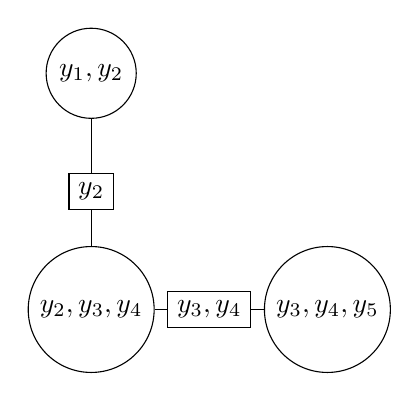
\begin{tikzpicture}[main/.style = {draw, circle}, sep/.style= {draw, rectangle}, node distance=1.5cm] 
			\node[main] (12)  {$y_1, y_2$};
			\node[sep] (2)  [below of=12]{$y_2$}; 
			\node[main] (234) [below of=2] {$y_2, y_3, y_4$};
			\node[sep] (34)  [right of=234]{$y_3,y_4$}; 
			\node[main] (345) [right of=34] {$y_3, y_4, y_5$};
			\draw[-] (12) -- (2);
			\draw[-] (2) -- (234);
			\draw[-] (234) -- (34);
			\draw[-] (34) -- (345);
		\end{tikzpicture}
		\caption{Junction Tree}
		\label{fig:iq-mp-exmp-jt}	
	\end{marginfigure}
Consider the JT shown in Figure \ref{fig:iq-mp-exmp-jt}. Note that we have edge potentials, and each clique has the product of such potentials present. Each node can send a message once it has messages from neighbors. \\
Initially, $C_1 = \{y_1, y_2\}$ or $C_3 = \{y_3, y_4, y_5\}$ can initiate the message passing since they have single neighbors. Thus, we have
\begin{enumerate}
	\item $C_1$ initiates message $m_{12\to234}(y_2) = \sum_{y_1} \psi_{12}(\mathbf y_{12})$ to $C_2 = \{y_2, y_3, y_4\}$.
	\item $C_3$ sends message $m_{345\to234}(\mathbf y_{34}) = \sum_{y_5}\psi_{345}(\mathbf y_{345})$ to $C_2$
	\item $C_2$ sends message $m_{234\to345} = \sum_{y_2} \psi_{234}(\mathbf y_{234})m_{12\to234}(y_2)$ to $C_3$
	\item $C_2$ sends message $m_{234\to12}(y_2) = \sum_{\mathbf{y_{34}}} \psi_{234}(\mathbf y_{234})m_{345\to234}(\mathbf y_{34})$ to $C_1$
\end{enumerate}
We also write that $\Prob(y_1) \propto \sum_{y_2} m_{234\to12}(y_2)$.
\end{exmp}
\begin{rem}[Intuition behind message passing]
Message from $c$ to $c'$ denotes the result of VE of potentials on the side of the tree that contains the clique $c$ but not $c'$ leaving only the separator variables $s = c\cap c'$.
\end{rem}
\subsection{Addition of Evidence}
In such queries, we have an evidence or conditioning set $\mathbf x_e$, and we need to find similar types of sub-queries shown before, i.e
\begin{enumerate}	\item $\Prob(x_1 | \mathbf{x}_e) = \sum_{x_2, \cdots, x_m} \Prob(x_1, \cdots, x_n| \mathbf{x}_e)$ \\
\item $\mathbf{x}^* | \mathbf{x}_e= \argmax_{x_1, \cdots, x_m} \Prob(x_1, \cdots, x_n | \mathbf{x}_e)$
\end{enumerate}
where $\{x_2, \cdots, x_m\} = V - \mathbf{x}_e - \{x_1\}$. The trick to add evidence is to change the potentials.
\begin{marginfigure}
	\centering
	\begin{tikzpicture}[main/.style = {draw, circle}] 
		\node[main] (y1)  {$y_1$}; 
		\node[main] (y2) [right of=y1] {$y_2$};
		\node[main] (y3) [right of=y2] {$y_3$};
		\node[main] (y6) [right of=y3] {$y_6$};
		\node[main] (y7) [right of=y6] {$y_7$};
		\node[main] (x1) [below of=y1] {$x_1$};
		\node[main] (x2) [below of=y2] {$x_2$};
		\node[main] (x3) [below of=y3] {$x_3$};
		\node[main] (x6) [below of=y6] {$x_6$};
		\node[main] (x7) [below of=y7] {$x_7$};
		\node at ($(y3)!.5!(y6)$) {\ldots};
		\draw[->] (y1) -- (x1);
		\draw[->] (y1) -- (y2);
		\draw[->] (y2) -- (x2);
		\draw[->] (y2) -- (y3);
		\draw[->] (y3) -- (x3);
		\draw[->] (y6) -- (x6);
		\draw[->] (y6) -- (y7);
		\draw[->] (y7) -- (x7);
	\end{tikzpicture}
	\caption{Sample HMM}
	\label{fig:iq-xe-hmm}	
\end{marginfigure}
\begin{exmp}[Viterbi Algorithm]
Consider the Hidden Markov Model shown in Figure \ref{fig:iq-xe-hmm}. Define edge potentials as $\Prob(y_i|y_{i-1})$ and $\Prob(x_i|y_i)$. Also, let the evidence variables be $\mathbf{x} = x_1, \cdots, x_n = o_1, \cdots, o_n$. We need to find the most likely values of the hidden state variables $\mathbf y = y_1, \cdots, y_n$, i.e
\[\argmax_\mathbf{y} \Prob(\mathbf y | \mathbf x = \mathbf o)\]
We redefine the potentials as
\[\psi_i(y_{i-1}, y_i) = \Prob(y_i|y_{i-1})\Prob(x_i=o_i|y_i)\]
\begin{marginfigure}
	\centering
	\begin{tikzpicture}[main/.style = {draw, circle}] 
		\node[main] (y1)  {$y_1$}; 
		\node[main] (y2) [right of=y1] {$y_2$};
		\node[main] (y3) [right of=y2] {$y_3$};
		\node[main] (y6) [right of=y3] {$y_6$};
		\node[main] (y7) [right of=y6] {$y_7$};
		\node at ($(y3)!.5!(y6)$) {\ldots};
		\draw[->] (y1) -- (y2);
		\draw[->] (y2) -- (y3);
		\draw[->] (y6) -- (y7);
	\end{tikzpicture}
	\caption{Sample HMM}
	\label{fig:iq-xe-rcg}	
\end{marginfigure}
Since we have fixed the observations of $x_i = o_i$, we have a 1D table instead of a 2D potential table. This gives the reduced chain graph as in Figure \ref{fig:iq-xe-rcg}. Now we use the message passing algorithm shown earlier, just replacing sum with max. For ease of calculation, only consider a three node chain, with the following probabilities:
\[\Prob(y_i = 0|y_{i-1}) = 
\begin{cases}
	0.9 &\text{if } y_{i-1} = 0 \\
	0.2 &\text{if } y_{i-1} = 1
\end{cases}
\]
\[\Prob(x_i = 0|y_{i}) = 
\begin{cases}
	0.7 &\text{if } y_{i} = 0 \\
	0.6 &\text{if } y_{i} = 1
\end{cases}
\]
Also, $\Prob(y_1 = 1) = 0.5$. Say our observations are
\[[x_1, x_2, x_3] = [0, 0, 0]\]
We want to calculate
\[\argmax \Prob(y_1, y_2, y_3 | x_1, x_2, x_3 = [0,0,0])\]
Now, we calculate the potential $$\psi_{12}(y_1, y_2)= \Prob(y_2|y_1)\Prob(x_1=0|y_1)\Prob(y_1)$$ 
\begin{center}
\begin{tabular}{cc|c|c|}
	& \multicolumn{1}{c}{} & \multicolumn{2}{c}{$\psi_{12}(y_1, y_2 ) $}\\
	& \multicolumn{1}{c}{} & \multicolumn{1}{c}{$0$}  & \multicolumn{1}{c}{$1$} \\\cline{3-4}
	\multirow{2}*{}  & $0$ & $0.9 \times 0.7 \times 0.5$ & $	0.1 \times 0.7 \times 0.5$ \\\cline{3-4}
	& $1$ & $0.2 \times 0.6 \times 0.5$ & $0.8\times 0.6 \times 0.5$ \\\cline{3-4}
\end{tabular}
\end{center}
Note that when we calculate $$\psi_{23}(y_2, y_3) = \Prob(y_3|y_2)\Prob(x_2=0|y_2)\Prob(x_3=0|y_3)$$
\end{exmp}
\begin{rem}[Approximate Inference]
Note the followings points:
\begin{itemize}
	\item[$\diamond$] Exact inference is NP hard. First define the tree width $w$ of a triangulated graph as one less than the size of the maximal clique. The complexity of exact inference is $\mathcal{O}(m^w)$.
	\item[$\diamond$] It is seen that real-life graphs produce large cliques on triangulation. For example, an $n\times n$ grid has a tree width of $n$. A Kalman filter on $K$ parallel state variables influencing a common observation variable has a tree width of size $K+1$.
\end{itemize}
\end{rem}
\subsection{Generalized Belief Propogation}
Here, we tr to run some kind of message passing algorithms on graphs which look like junction trees. Instead of creating an exact JT which satisfies the running intersection property, we try to create a cluster graph with two relaxations - 
\begin{enumerate}
	\item The nodes are arbitrary clusters instead of cliques in the chordal graph. We only ensure that all potentials are subsumed.
	\item Instead of adding separator nodes, we add a subset of intersecting variables so as to satisfy the running intersection property.
\end{enumerate}
\begin{exmp}
Consider the JT creation in Example \ref{exmp:jt-creation}. For that graph, we see that we get maximal clique size of 3. Suppose we want to maintain a clique size of 2. 
\begin{marginfigure}
	\centering
	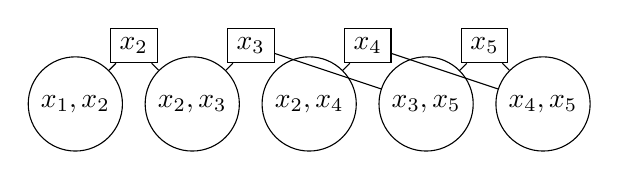
\begin{tikzpicture}[main/.style = {draw, circle}, sep/.style={draw, rectangle}, node distance=1.05cm] 
		\node[main] (12)  {$x_1, x_2$}; 
		\node[sep] (2) [above right of=12] {$x_2$};
		\node[main] (23) [below right of=2] {$x_2, x_3$}; 
		\node[sep] (3) [above right of=23] {$x_3$};
		\node[main] (24) [below right of=3] {$x_2, x_4$}; 
		\node[sep] (4) [above right of=24] {$x_4$};
		\node[main] (35) [below right of=4] {$x_3, x_5$}; 
		\node[sep] (5) [above right of=35] {$x_5$};
		\node[main] (45) [below right of=5] {$x_4, x_5$}; 
		\draw[-] (12) -- (2);
		\draw[-] (23) -- (2);
		\draw[-] (23) -- (3);
		\draw[-] (35) -- (3);
		\draw[-] (24) -- (4);
		\draw[-] (45) -- (4);
		\draw[-] (35) -- (5);
		\draw[-] (45) -- (5);
		\end{tikzpicture}
	\caption{Factor Graph}
	\label{fig:iq-gbf-fg}	
\end{marginfigure}
We create a \textit{factor graph} such that the nodes of the factor graph correspond to the edge potentials given. The cluster/factor graph will be as shown in Figure \ref{fig:iq-gbf-fg}. Note that factor graphs are special kinds of cluster graphs.
\end{exmp}
Belief propogation algorithms are approximate message passing algorithms, and differ in the order of sending of messages. Note that in general graph can have loops and thus we can't apply tree-based two phase methods. \\
\noindent Variants of scheduling order of propogating beliefs are - 
\begin{enumerate}
	\item Simple loopy belief propogation
	\item Tree-reweighted message passing
	\item Residual belief propogation
\end{enumerate}
There are other classes too, which are
\begin{enumerate}
	\item Sampling
	\item Combinatorial Algorithms
	\item Greedy algorithms: relaxation labeling
	\item Variatinal methods - mean-field \& structured mean-field
	\item Linear and Quadratic Programming based approaches
\end{enumerate}